%for a more compact document, add the option openany to avoid
%starting all chapters on odd numbered pages
\documentclass[12pt]{cmuthesis}

% This is a template for a CMU thesis.  It is 18 pages without any content :-)
% The source for this is pulled from a variety of sources and people.
% Here's a partial list of people who may or may have not contributed:
%
%        bnoble   = Brian Noble
%        caruana  = Rich Caruana
%        colohan  = Chris Colohan
%        jab      = Justin Boyan
%        josullvn = Joseph O'Sullivan
%        jrs      = Jonathan Shewchuk
%        kosak    = Corey Kosak
%        mjz      = Matt Zekauskas (mattz@cs)
%        pdinda   = Peter Dinda
%        pfr      = Patrick Riley
%        dkoes = David Koes (me)

% My main contribution is putting everything into a single class files and small
% template since I prefer this to some complicated sprawling directory tree with
% makefiles.

% some useful packages
\usepackage{times}
\usepackage{fullpage}
\usepackage{graphicx}
\usepackage{amsmath}
\usepackage{cite}
\usepackage{multirow}
\usepackage[numbers,sort]{natbib}
\usepackage[pageanchor=true,plainpages=false, pdfpagelabels, bookmarks,bookmarksnumbered,
%pdfborder=0 0 0,  %removes outlines around hyper links in online display
]{hyperref}
\usepackage{setspace}
\usepackage{subfigure}
\usepackage{titlesec}
\DeclareMathOperator*{\argmin}{arg\,min}
\newcommand\addtag{\refstepcounter{equation}\tag{\theequation}}
\titleformat{\chapter}[hang] 
{\normalfont\LARGE\bfseries}{\chaptertitlename\ \thechapter:}{1em}{}

% Approximately 1" margins, more space on binding side
%\usepackage[letterpaper,twoside,vscale=.8,hscale=.75,nomarginpar]{geometry}
%for general printing (not binding)
\usepackage[letterpaper,twoside,vscale=.8,hscale=.75,nomarginpar,hmarginratio=1:1]{geometry}

% Provides a draft mark at the top of the document. 
\draftstamp{\today}{DRAFT}

\begin {document} 
\frontmatter

%initialize page style, so contents come out right (see bot) -mjz
\pagestyle{empty}

\title{ %% {\it \huge Thesis Proposal}\\
{\bf Inharmonicity Regression against Pitch for Automatic Guitar Tablature Transcription}}
\author{Jonathan Michelson}
\date{May 2017}
\Year{2017}
\trnumber{}

\committee{
Dr. Richard Stern, Dr. Thomas Sullivan \\
}

\support{}
\disclaimer{}

% copyright notice generated automatically from Year and author.
% permission added if \permission{} given.

%\keywords{Stuff, More Stuff}

\maketitle

%\begin{dedication}
%For my dog
%\end{dedication}

\pagestyle{plain} % for toc, was empty

%% Obviously, it's probably a good idea to break the various sections of your thesis
%% into different files and input them into this file...

%\doublespacing
\begin{abstract}
We propose and evaluate an additional method for inharmonicity-based automatic tablature transcription. First, for each string, we linearly regress note pitches against their inharmonicity estimates. Then we use these learned regressions to predict string labels of unseen guitar notes: the system classifies a pitch's string label as the one whose regression approximates the note's inharmonicity with minimal error. Given the tuning of the guitar that produced the unseen note, we infer its associated tablature, which allows for further string classification refinement by rejecting and reassigning implausible fret assignments. Average F1-scores achieved with this system for classical, acoustic, and electric guitars were $0.43$, $0.71$, and $0.62$ respectively. We also derive and evaluate an inharmonicity scaling factor to allow for transcription of arbitrarily-tuned guitars, provided the tuning is known. With this feature, our system performance improves by $17.5\%$ on alternate-tuned guitars on average, compared to performance with no tuning compensation.

\end{abstract}
%\singlespacing

\begin{acknowledgments}
My advisors are cool.
\end{acknowledgments}



\tableofcontents
\listoffigures
\listoftables

\mainmatter

%% Double space document for easy review:
%\renewcommand{\baselinestretch}{1.66}\normalsize

% The other requirements Catherine has:
%
%  - avoid large margins.  She wants the thesis to use fewer pages, 
%    especially if it requires colour printing.
%
%  - The thesis should be formatted for double-sided printing.  This
%    means that all chapters, acknowledgements, table of contents, etc.
%    should start on odd numbered (right facing) pages.
%
%  - You need to use the department standard tech report title page.  I
%    have tried to ensure that the title page here conforms to this
%    standard.
%
%  - Use a nice serif font, such as Times Roman.  Sans serif looks bad.
%
% Other than that, just make it look good...
\doublespacing
\noindent
\chapter{Introduction} 
\section{Guitar and Tablature} The guitar is a popular musical instrument whose family comprises a diverse collection of stringed instruments. Its most prominent classes are the acoustic, classical, and electric guitars, and intraclass variation in characteristics such as body shape, string material, and amplification mode is high. Despite this diversity, the majority of guitar configurations have six strings tuned to $E2$ ($82$Hz), $A2$ ($110$Hz), $D3$ ($147$Hz), $G3$ ($196$Hz), $B3$ ($247$Hz), and $E4$ ($330$Hz). To play, a performer presses these strings with one hand against the neck's metal frets, each of which increase the string's pitch by one half-step, while strumming or plucking them with the other hand. Guitars typically have upwards of 20 frets, allowing for versatile musical passage realizations along the fretboard.

A consequence of this is liberal pitch overlap between neighboring strings. Conventional music scores that represent passages as notes and chords therefore fail to communicate fretboard position. This ambiguity renders scores unfit for guitar students trying to learn more skillful placement of scales and arpeggios, or for enthusiasts trying to decrypt the fretboard positions used on recordings of virtuosic players' riffs. Figure~\ref{fig:score-tabs} illustrates this ambiguity.

Tablature, on the other hand, is an alternative music notation that doesn't suffer from the one-to-many mapping of scores. The staff, instead of representing pitch as in classical scores, depicts a birds-eye view of the guitar neck from the performer's perspective. Each of the six horizontal lines signify a corresponding string on the guitar, and numbers on each line specify the fret to be played. Time progresses from left to right as in scores. 

\begin{figure}[h] 
\label{fig:score-tabs}
\centering
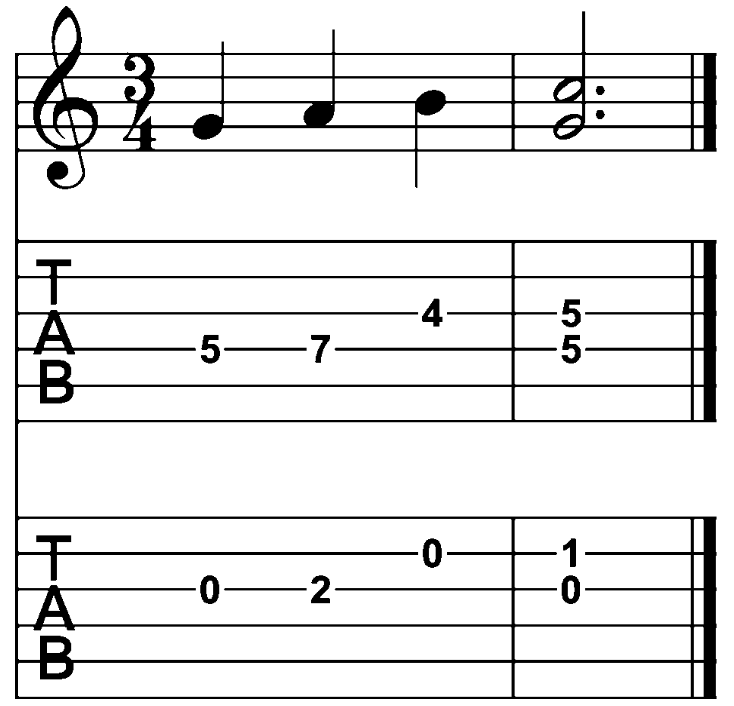
\includegraphics[scale=0.8]{score-tabs}
\caption{Musical score and two identical realizations of that score in tablature notation. Figure taken from~\cite{barbanchoi2012}.}
\end{figure}

Tablature (tabs for short) is widely popular for a number of likely reasons. Its accessibility and intuition are attractive to those without formal musical training; learning from a pictorial representation of one's instrument must seem more attractive to beginners than learning musical theory foundations and decoding scores. And because tabs are easily encodable and interpretable with simple ASCII characters, authoring them isn't limited to those with knowledge of any sort of tab-specific generation program, unlike with scores.~\cite{macrae2010}.

Accurate tablature transcription is a fairly tedious task, however. Dependable tabs containing few errors typically require a seasoned musician's careful listening to an audio recording, and possibly video recordings if available too. Reliable automation of this transcription task would benefit the guitar student community by expediting quality tab generation and unearthing fretboard positions of guitar riffs in songs for which accurate tabs don't yet exist. Recent technologies proposed to encourage proliferation of accessible tab transcription systems, such as web framework Robotaba~\cite{burlet2013}, demonstrate a desire among MIR researchers to see this theoretically mature but practically nascent field mature into student-benefitting applications. Closely related to tab transcription is the task of string classification: producing the correct tablature is straightforward if the guitar's tuning is known and the correct string labels are identified. In chapter~\ref{lit-review}, we present much of the work that's been done in these fields.

\section{Inharmonicity} Inharmonicity is a key feature in many string discrimination systems~\cite{barbanchoi2012,abesser2012,dittmar2013,kehling2014}. Because its termination points are not perfectly rigid~\cite{fletcher1998}, a vibrating string's harmonic partials are skewed upward in frequency according to: 
\begin{equation}
f_k = kf_{0}\sqrt{1+\beta k^2} \label{eq:fk}
\end{equation}
where $f_k$ is the $k$th harmonic of fundamental $f_0$ and $\beta$ is the string's inharmonicity, defined by
\begin{equation}
\beta = \frac{\pi Q d^4}{64 T l^2}. \label{eq:beta}
\end{equation}
In words, the inharmonicity $\beta$ of a vibrating string is a dimensionless quantity that depends on the string's Young's modulus $Q$, diameter $d$, tension $T$, and vibrating length $l$, and which scales the degree of deviation of the string's $k$th partial according to equation~(\ref{eq:fk}). See Figure~\ref{fig:skew}. Note that for an ideally harmonic string, $\beta = 0$ and~(\ref{eq:fk}) reduces to $f_k = kf_0$, aligning with intuition about harmonics' ideal locations in frequency as simply integer multiples of the fundamental.

\begin{figure}[h] \label{fig:skew}
\centering
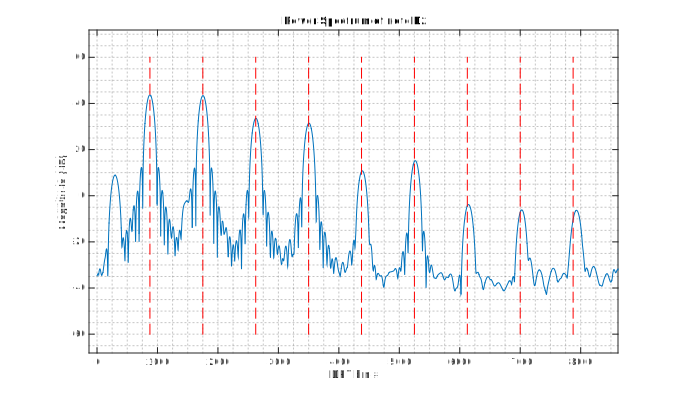
\includegraphics[scale=0.65]{skew}
\caption{Power spectrum of note D2 plucked on an electric guitar at string 5 and fret 5. Red dashed lines are drawn at integer multiples of the fundamental. Note the rightward skew of the measured partial peaks.}
\end{figure}

%This phenomenon is audible in lower pitch registers because of the necessity of thicker longer strings, and is therefore important for increased realism of synthesized instrument sounds~\cite{jarvalainen2003,fletcher}. Interestingly, not critically audible for acoustic guitar sounds though~\cite{karjalainen}. 

Inharmonicity's suitability for the string discrimination task can be understood through equation~(\ref{eq:beta}). The six strings of any guitar necessarily exhibit different combinations of $Q$, $d$, and $T$ due to varying thicknesses, material, and tuning. Each string therefore has an "inharmonic signature" which presumably distinguishes it from the others. Capturing the pattern of a string's inharmonicity variation along its frets should thus reveal sufficiently identifying information.



\noindent
\chapter{Literature Review} \label{lit-review}
\section{Inharmonicity Estimation}
Estimation of inharmonicity using pitch extraction techniques was first attempted by Galembo in 1979 and 1986~\cite{galembo1979,galembo1987}. Several additional methods have been proposed since then. In 1994, Galembo~\cite{galembo1994} hypothesized a connection between partials-based fundamental pitch estimates and the degree of inharmonicity in a spectrum. They specifically investigated cepstral analysis and a variant of the harmonic product spectrum method applied to both synthetic tones and recorded piano notes. They found that, because these two techniques leverage periodicity in the frequency domain to produce their pitch estimates, inharmonicity influenced the quality of their estimates in a deterministic manner: more inharmonicity produced wider, less focused pitch estimates lobes, and from quantifying this relation an inharmonicity could be obtained.
 
 The same authors in~\cite{galembo1999} introduced another method in 1999, dubbed the inharmonic comb filter (ICF) method. To estimate a note's inharmonicity, they first applied sets of comb filters to the note's spectrum. The locations of the comb filters' notches were parametrized with a range of inharmonicity values that sufficiently sampled the note's expected inharmonicity range. The ICF whose inharmonicity best matched that of the note would produce the output with lowest spectral energy, since its notches best aligned with the inharmonic note partials. The inharmonicity parameter associated with this output-maximizing ICF was thus selected as the estimate.
 
Rauhala~\cite{rauhala2007} introduced an efficient procedure in 2007 that iteratively catalogued estimates of the partial frequencies' deviations and returned increasingly better estimates of the inharmonicity. The algorithm, aptly referenced as the partial frequency deviations (PDF) method, is initialized with a reasonable first estimate of inharmonicity, and then the note's spectrum is searched for partial peaks. Differences are measured between the locations of these discovered peaks and those of the expected peaks, and the aggregate deviation trend is used to refine the inharmonicity estimate -- a majority of positive differences implies the inharmonicity should be reduced, and a majority of negative differences implies the opposite.

In 2009, Hodgkinson~\cite{hodgkinson2009} proposed a yet more efficient and accurate algorithm, named median-adjustive trajectories (MAT). Their routine exploits the fact that inharmonicity can be estimated with any two partials and their corresponding indices in the harmonic series. Pairs of low-index partials are first considered, since they're minimally affected by inharmonic skew and therefore have high location reliability. With these initial inharmonicity estimates, additional partials are collected and used to refine the previous inharmonicity estimates, with which more partials are located, so on and so forth. MAT was the inharmonicity estimation routine employed in this work, and is discussed at length in Chapter~\ref{experiments}.

Three years later, Barbancho~\cite{barbanchoi2012} introduced another PFD-based approach as part of a guitar tablature transcription system. They started by cataloguing the first 10 partials' deviations, then fitting a polynomial to the PFD curve. They derived the relation between the polynomial's coefficients and the inharmonicity, and returned an initial inharmonicity estimate according to this derivation. Then using this inharmonicity to aid in their search for higher-index partials, they catalogued a larger number of partials' deviations than that of the first iteration, and performed the same polynomial fit and inharmonicity derivation routine. This would refine the inharmonicity estimate, allowing for ever-increasing numbers of partials for which to search.

Also in 2012, Abesser~\cite{abesser2012} successfully used parametric spectral modeling, again in the context of a guitar tablature transcription system. To estimate the inharmonicity of a plucked guitar note, they modeled each audio frame with the autoregressive (AR) filter that best approximated its spectral content. They obtained the poles' locations and the ideal harmonics' locations, and like Barnbancho~\cite{barbanchoi2012} fit the PFD curve with a polynomial from whose coefficients an inharmonicity estimate could be derived.

\section{Automatic Tablature Transcription}
[in-progress]
%A subtle distinction is worth noting between methods that focus on tablature generation versus tablature transcription. In the former task, the goal is generally production of a plausible tablature which is optimal in some sense. Performance metrics could be amount of agreement with human-generated tabs (with no guarantee on their correctness), or heuristic cost functions that characterize the quality of the tab (e.g. predicted mechanical difficulty, spatial compactness, etc.). In the latter task, the goal is exact recovery of the original tablature that produced the observed audio. In this case, the performance metrics are classification accuracies derived from the predicted vs. true string and fret labels of annotated guitar recordings.

%A number of authors have worked with tablature generation from music scores. Radisavljevic~\cite{radisav2004} and Radicioni~\cite{radicioni} create directed acyclic graphs that model a score's candidate fretboard positions, and return the final transcription as the most optimal path. Their cost functions incorporate combinations of the tablature's mechanical difficulty and musicality. Tuohy~\cite{asdf} employs neural nets and genetic algorithms to transform score into tablature. 

%Audio-based transcription systems are numerous as well. Yaezawa~\cite{yaezawa} extracted pitch and melody information from guitar recordings, and computed an optimal fingering based on plausible multipitch estimation results. Gagnon~\cite{gagnon2003} proposed using neural networks to deduce general fretboard region position and number of strings playing. Sayegh~\cite{sayegh} introduced the Viterbi graph search as a solution to the stringed-instrument transcription problem for monophonic musical passages. Burlet~\cite{burlet} extended this to polyphonic passages.  

%The tablature transcription task is also well studied. Ogrady -- hexaphonic pickup.
%Gagnon\cite{2003} trained neural networks to detect general hand position along the neck and number of played strings for a given recording.
%In Barbancho et al. ~\cite{barbancho2009}, the authors attempt guitar string classification using features such as nontonal spectrum, etc., but achieve discouraging results.
%Barbancho et al. ~\cite{barbanchoi2012}
%Estimation typically involves searching a note's spectrum for peaks in the vicinity of multiples of the fundamental, then cataloguing located peaks' deviations from their ideal locations, and fitting a polynomial -- one of whose coefficients corresponds to a good estimate of the inharmonicity -- to the deviations curve. Barbancho~\cite{barbanchoi2012} achieves good tablature transcription using open-strings' inharmonicities and checking unknown notes' inharmonicities against those of string candidates. In various supervised classification approaches~\cite{abesser2012, kehling2014, dittmar2013}, the authors achieve good string transcription after training on standard-tuning guitar audio and using inharmonicity as one of their features.

\noindent
\chapter{Inharmonicity Regression against Pitch}
\section{Motivation}
Barbancho~\cite{barbanchoi2012} realized that inharmonicity varies in a deterministic manner with respect to fret positions along a given string. Specifically, they showed that the inharmonicity $\beta(s,n)$ of a note produced by string $s$ at fret number $n$ could be expressed in terms of the inharmonicity of the open-string note $\beta(s,0)$ according to:
\begin{equation} 
\label{eq:beta-traj}
\beta(s,n) = \beta(s,0)2^{\frac{n}{6}}
\end{equation}
In other words, the variation in inharmonicity along a given string can be expressed simply in terms of its open-note inharmonicity, effectively defining a restricted trajectory along which the inharmonicity must vary. Figure~\ref{fig:beta-trajectories-ag} illustrates these trajectories.

\begin{figure}[h] 
\label{fig:beta-trajectories-ag}
\centering
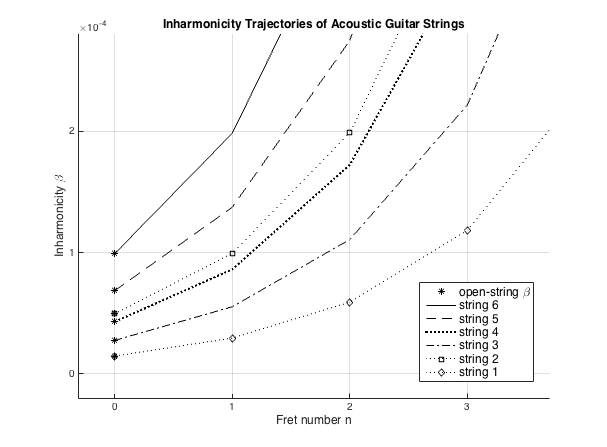
\includegraphics[scale=0.70]{beta-trajectories-ag}
\caption{Example inharmonicity trajectories of acoustic guitar strings. Only frets 0 (open-string) through 3 are shown. Observe the restriction to the exponential trajectory defined by equation~\eqref{eq:beta-traj}.}
\end{figure}

With this, they were able to successfully transcribe string and fret number of an unknown guitar note, provided they had access to recordings of its guitar's open-strings. First, they estimated these open-notes' inharmonicities. Then to classify an unknown note, they estimated its fundamental pitch and selected as candidate strings those that could plausibly produce that pitch. Next, they inferred the corresponding frets on which the note could be played for each candidate string, and used these string-fret candidate numbers in equation~\eqref{eq:beta-traj} to obtain expected inharmonicity values of the unknown note for each candidate string. Lastly, they measured the extent of agreement between the note's measured partials' locations and those of each candidate string given its expected inharmonicity. They performed this similarity measurement by traversing the note's spectrum according to each candidate string's inharmonicity, counting the number of partials measured in search windows centered about the string's inharmonicity trajectory. They found that, indeed, the inharmonicity trajectory of the string on which the note was truly plucked would yield higher counts than those of the imposter strings, and in this fashion impressive transcription results could be obtained. Their work demonstrated the sufficiency of inharmonicity as a discriminating feature.

This work capitalizes further on their trajectory realization. If we reconsider equation~\eqref{eq:beta-traj} in terms of MIDI pitch number $m$ instead of fret number $n$, we obtain
\begin{equation}
\beta(s,m) = \beta(s,m_{os})2^{\frac{m-m_{os}}{6}},
\end{equation}
where $m_{os}$ is the open-string pitch of string $s$. The exponential trajectory is maintained since incrementing both fret number and MIDI pitch number accomplishes an equivalent increase in fundamental frequency. Figure~\ref{fig:beta-v-midi} illustrates the trajectories in terms of MIDI pitches.

\begin{figure}[h] 
\label{fig:beta-v-midi}
\centering
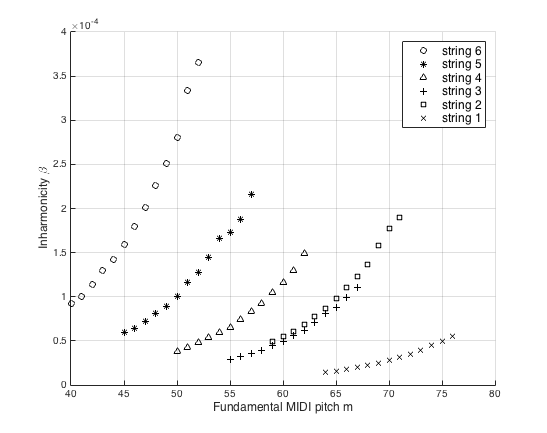
\includegraphics[scale=0.7]{beta-v-midi}
\caption{Trajectories of inharmonicity estimates for the strings of RWC acoustic guitar 111AG. Note the same exponential pattern as in Fig.~\ref{fig:beta-trajectories-ag} and the increased segregation since notes and their inharmonicities are now plotted against their fundamental instead of their fret number.}
\end{figure}

 Now if we consider the log-inharmonicity $\beta_{l}(m)$ of a note, we see that
\begin{equation}
\beta_l(m) = \log_2\beta(s,m) = \log_2[\beta(s,m_{os})2^{\frac{m-m_{os}}{6}}]
\end{equation}
\begin{equation}
\beta_l(m) = \log_2\beta(s,m_{os}) + \frac{m-m_{os}}{6}
\end{equation}
\begin{equation}
\beta_l(m) = (\log_2\beta(s,m_{os})-\frac{m_{os}}{6}) + (\frac{1}{6})m.
\end{equation}
The term $\log_2\beta(s,m_{os})-\frac{m_{os}}{6}$ is constant for each string (assuming its tuning is constant throughout a performance), so if we substitute it with $w_0$ and let $w_1 = \frac{1}{6}$, we obtain
\begin{equation}
\beta_l(m) = w_0 + w_1m,
\end{equation}
which shows us that the log-inharmonicity trajectory is linear with respect to MIDI pitch. See Figure~\ref{fig:log-beta-v-midi}.

\begin{figure}[h] 
\label{fig:log-beta-v-midi}
\centering
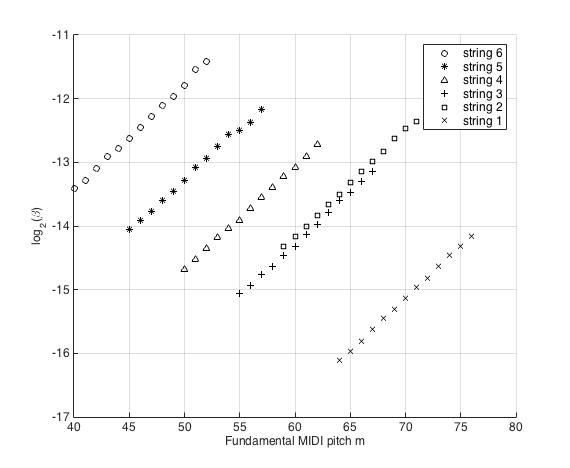
\includegraphics[scale=0.7]{log-beta-v-midi}
\caption{Trajectories of log-inharmonicity estimates of same guitar as Fig.~\ref{fig:beta-v-midi}}
\end{figure}

Instead of tallying the number of coincident partial peaks of the unknown note and candidate strings, we propose characterizing each candidate string by its log-inharmonicity trajectory and classifying a note as belonging to the string whose regression best explains (error-wise, probability wise, etc.) the note's inharmonicity. This is an algorithmically simple approach, requiring only a linear regression and a distance metric for classification. Additionally, this method is governed by the intuitive constraint of inharmonicity trajectory: notes played on a given string can exhibit only a set of inharmonicities, so the note with inharmonicity closest to that set likely belongs to that string. %Barbancho's assessment of inharmonicity agreement, but, in tallying a note's and candidate strings' shared peaks, does so in a slightly more ad-hoc way. (refine this...)

Barbancho~\cite{barbanchoi2012} also assessed transcription performance when using averages of open-string inharmonicites across the guitars in their dataset. By doing this, they effectively approximated their transcription performance on guitars the system has never before seen. Though their accuracy degraded slightly, a good demonstration of solely inharmonicity-based string classification for unseen guitars was still demonstrated. We're interested in how much, if at all, the robustness of our regression approach differs from that of Barbancho's~\cite{barbanchoi2012} and other researchers' systems.

\section{Inharmonicity Estimation}
Here, we discuss the algorithm we median adjustive trajectories (MAT) algorithm~\cite{hodgkinson2010} we employed for inharmonicity estimation. If we consider equation~eqref\

\section{String Classification}
We collect all notes with common string labels in our training data, and we perform linear regression of their inharmonicities $\beta$ against their fundamental pitches $m$ (in MIDI note number format). We do this for each string label. Let $s \in \{1,2,3,4,5,6\}$ be the string label to which each training note is assigned, and $N_s$ be the number of notes we have belonging to string label $s$. If we let $\mathbf{x}_s^{(i)} = [1, m_s^{(i)}]^T$ represent the $i$th note with fundamental pitch $m^{(i)}$ belonging to string $s$ , and $\beta_s^{(i)}$ be the inharmonicity of the $i$th note belonging to string $s$, we can solve
\[
\mathbf{w}_s = \argmin_{\mathbf{w}}{\sum_{i=1}^{N_s}{(\beta^{(i)}_s - \mathbf{w}^T\mathbf{x}^{(i)}_s)^2}}\addtag
\]
which yields the weight vector $\mathbf{w}_s$ that minimizes the sum of squared error between the measured and predicted inharmonicities of the notes belonging to string $s$. Figure~\ref{fig:regressions} illustrates these learned regressions for the electric guitar. Now that we've learned a characterization of each strings' inharmonic quality, we can use this to predict unseen notes.

\begin{figure}[h] 
\label{fig:regressions}
\centering
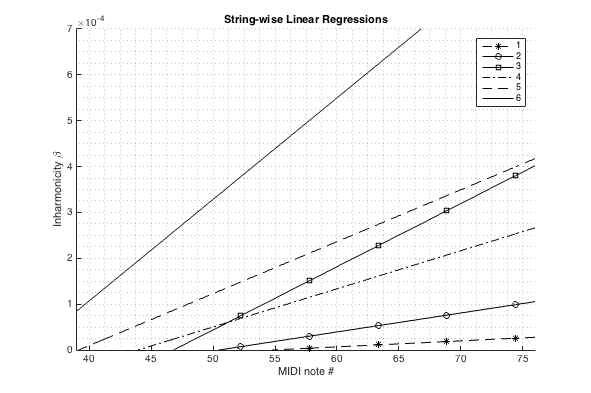
\includegraphics[scale=0.8]{regressions}
\caption{Regressions of inharmonicity against pitch for each string, learned from multiple RWC electric guitar recordings. String number with corresponding line type is displayed in the top-right legend.}
\end{figure}

For prediction, we take the $n$th note in our test set, characterized by tuple $(m^{(n)},\beta^{(n)})$ where $m^{(n)}$ is its MIDI pitch number and $\beta^{(n)}$ is its inharmonicity. We'd like to transform this into another tuple $(s^{(n)},f^{(n)})$ corresponding to the appropriate string and fret to which this unknown note should be assigned. A straightforward solution is to assign to $s^{(n)}$ the index $j$ of the regression weights $\mathbf{w}_j$ whose predicted inharmonicity $\hat\beta_j$ approximates the measured inharmonicity $\beta^{(n)}$ with least error. More formally, we solve 
\[
s^{(n)} = \argmin_{j}{(\beta^{(n)} - \hat{\beta}_{j})^2} \addtag
\]
where $\hat\beta_j$ is the inharmonicity prediction of string $j$ according to its learned regression, given by
\[
\hat{\beta}_{j} = \mathbf{w}_{j}^T\mathbf{x}^{(n)} \addtag
\]
where, as before, $\mathbf{x}^{(n)} = [1, m^{(n)}]^T$. See Figure~\ref{fig:classification} for a graphical illustration of this process.

\begin{figure}[h] 
\label{fig:classification}
\centering
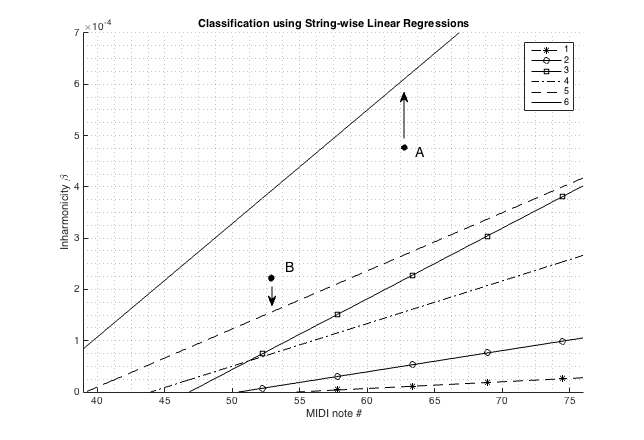
\includegraphics[scale=0.75]{classification}
\caption{Classifying two new notes A and B using the learned inharmonicity regressions. Note A is assigned to string 6, since its regression is closest to A's inharmonicity estimate. Note B's location in inharmonicity-pitch space is closest to string 5's regression, so it is assigned to that string.}
\end{figure}

\section{Tablature Conversion and Refinement}
To generate tablature, we still need to infer notes' fret positions. This is a trivial task provided we know the tuning $\mathbf{t} = [m_1, m_2, m_3, m_4, m_5, m_6]^T$ of the unknown guitar, where $m_s$ is the MIDI pitch number of the open note on string $s$. Because we already have an estimate of the $n$th unknown note's MIDI pitch $m^{(n)}$, simply taking the difference between $m^{(n)}$ and its assigned string's open pitch $m_s$ yields the fret on which the note was played; each fret on a guitar increases the string's pitch by one half-step, or equivalently the MIDI pitch number by one integer.

The merit of this fret assignment routine is dependent on the string assignment. If an incorrect string is assigned to note $n$, the fret assignment will be consistent with the string but necessarily incorrect as well. In some cases, an incorrect string assignment could yield a negative fret assignment, which is nonsensical. A simple fix that intuitively fits the proposed regression model is to reassign the string label to that of the regression of next least prediction error. This harmonizes well with the reality that the regressions are only generally predictive, since they're learned from averages of the training data; for the cases in which nonsensical strings are selected, we attribute the error to the deviant behavior of the test note's inharmonicity, and conclude that the next most sensible label reassignment is that of the string whose regression, on average, best explains the test note's inharmonicity. This process can be iterated for as long as fret assignments continue being nonsensical, until all string reassignments are exhausted. A similar procedure is employed by Abesser~\cite{abesser2012} under the name plausibility filtering.

\section{Tuning Compensation}
Though standard tuning is the most common pitch configuration of six-string guitars, there exist numerous other tunings in which performers often play. Aside from altering the musicality of the instrument, alternate tunings complicate the transcription process by introducing uncertainty about the open-string pitches. They distort inharmonicity-based methods, since the tensions $T$ of alternately-tuned guitar strings differ from those in standard-tuned strings, thereby affecting estimation of the inharmonicity. 

Current string classification systems don't address this degree of freedom. The method proposed by Barbancho~\cite{barbanchoi2012} is technically tuning-invariant, but requires access to recordings of the the test guitar's open strings and so isn't considered a classifier here. Other supervised learning systems~\cite{kehling2014, dittmar2013, abesser2012} are trained and evaluated only on standard-tuning guitars.

A possible approach to augment inharmonicity-based string classifiers with tuning-invariant performance is to simply introduce a scaling factor on the expected inharmonicity. The fundamental frequency $f_0$ of an ideal vibrating string is related to its tension $T$ according to
\begin{equation}
f_0 = \frac{1}{2L}\sqrt{\frac{T}{\mu}}
\end{equation}
where $L$ is string length and $\mu$ is its density. From this, we can see that
\begin{equation}
T \propto f_0^{2} \addtag
\end{equation}
Recognizing that for a change in pitch of $m$ semitones, the equivalent change in frequency is $2^{\frac{m}{12}}$, we see that the proportional change in tension (with all other factors constant) is
\begin{equation}
T \propto 2^{\frac{m}{6}}f_0^2, \addtag
\end{equation}
and that the resulting inharmonicity is therefore
\begin{equation}
\beta = (2^{-\frac{m}{6}}) \frac{\pi Q d^4}{64 T l^2}. \addtag
\end{equation}
If we're given the alternate tuning of the unseen guitar and we have pre-computed inharmonicity regressions of other standard-tuned guitars, we should be able to compensate our predictive regressions by a factor of $2^{-\frac{m}{6}}$ and expect more accurate transcription. This is a straightforward modification for any inharmonicity-exploiting classifier. We report our results with this modification in the next chapter.

\noindent
\chapter{Experiments and Results}
\label{experiments}
%We used subsets of the Real World Corpus' Music Instrument Database (RWC-MDB-I)~\cite{goto2003}, subsets of the Fraunhofer Institute for Digital Media Technology's Semantic Music Technologies guitar dataset (IDMT-SMT)~\cite{asdf}, and personal recordings of an electric guitar to conduct our experiments. 

We used subsets of the Real World Corpus' Music Instrument Database (RWC-MDB-I)~\cite{goto2003} and personal recordings of an electric guitar to conduct our experiments. 

Our RWC subset comprised nine guitar recordings (three classical, three acoustic, and three electric), each of which were performed numerous times with varying permutations on certain musicality parameters (playing style, dynamic level, pickup selection). The performances themselves were simply clean, isolated, monophonic enumeration of every fret (from open-string to 12th fret) on every string (from string 6 to string 1), constituting 78 total note plucks per audio file. The resolution is 16 bits per sample, at 44.1kHz. Labels of strings and frets are thus obtained by their location of occurrence in the recording. The classical guitars recorded were a Stafford, a Sakurai Kohno Professional-J, and a Yuichi Imai YJ-II; the three acoustic guitars captured were an Ovation, a Yamaha APX, and Yairi WY1; the electric guitars featured were a Fender Stratocaster, an Aria PE, and an Ibanez Artcore.

%The IDMT-SMT guitar dataset focuses on electric guitars, and boasts standardized licks performed across its sample instruments. The bit depth here is 24, with sampling rate equal to 44.1kHz. The subset we used featured six short licks (each between 10 and 30 notes), each of which were captured on three electric guitars: an Aristedes 010, a Fender Stratocaster, and a Gibson Les Paul. Transcriptions which included string and fret labels were saved as accompanying .xml files.

We also recorded a Fender Telecaster at 16 bits and 44.1kHz in the same vein as the RWC database: string and fret enumeration, totaling 78 notes per recording. We captured various tunings: standard, "DADGAD" (in which the open pitches of strings 6 through 1 are given in its name), "WSU" (whole-step up), and "WSD" (whole-step down), and performed each one with a pick at center pickup orientation and at a similar moderate dynamic level. Hardware included a Focusrite Saffire Pro 24 into a 2011 Macbook Pro running Logic. No other musicality parameters were captured; we focused on tuning variance here.

Our first experiment was a benchmark comparison of our similarity metric (residual error of each string's trajectory) to that of Barbancho (coincident partial peaks tally). We estimated inharmonicity and fundamental pitch of labeled open-string notes for our RWC evaluation guitar, then for each remaining fretted note, compiled a list of candidate string-fret positions from which the note could have been generated. For each candidate string, we obtained its appropriate theoretical fretted inharmonicity value by traversing the log-inharmonicity trajectory the as discussed in -----. The residual error between each test note's inharmonicity and each candidate strings' theoretical inharmonicity is computed, and the string whose index most closely predicts this test note's inharmonicity is returned as the string assignment. Table~\ref{tab:overall-results-RWC} summarizes the results from our first experiment. Guitar type abbreviations are as follows: CG is classical guitar, AG is acoustic guitar, EG is electric guitar. We conducted two trials per guitar type.

An aspect of this linear trajectory method is that it allows for string-wise linear regression of the full labeled recording data. We wanted to assess whether regressing inharmonicity empirically rather than theoretically (i.e., on open-string inharmonicity trajectory traversal) would produce more accurate transcriptions, so our next experiment tests this. First we assessed the quality of fit of both the theoretical trajectory and the empirical regression with $r^2$ determination coefficients. Then we performed the same classification experiment, and report the results below.

the merit of obtaining string-wise inharmonicity regressions from the ful


 %For the first trial, the regressions we used for prediction were obtained from all three guitar types, hence the column title "all." For the second trial, the regressions we used for prediction were obtained from only the guitar type for which we were predicting, hence the second column title name. 

%The F1-scores displayed were obtained in the following manner. Each guitar type featured three different guitars, e.g. the classical guitar type comprised recordings of CG1, CG2, and CG3. For each featured guitar, we performed classification and tabulated F1-scores for its strings. We then string-wise averaged the three featured guitars' F1-scores, and these are the results displayed in Table~\ref{tab:resultsRWC}.


\begin{table}
\begin{center}
\begin{tabular} {||c||c|c|c||c|c|c||}
\hline
\multicolumn{7}{|c|}{\bf{Transcription Accuracies}} \\
\hline
 & \multicolumn{3}{|c|}{Guitar-specific $\beta$'s} & \multicolumn{3}{|c|}{Guitar-averaged $\beta$'s}\\
\hline
Guitar & PFT & $\log_{2}\beta$ traj. & $\log_{2}\beta$ regr. & PFT & $\log_{2}\beta$ traj. & $\log_{2}\beta$ regr.\\
\hline
Classical CG091 & 0.96 & 0.9792 & 0.9553 & 0.91 & 0.9792 & 0.9553\\
\hline
Classical CG092 & 1.00 & 0.9189 & 0.8982 & 0.99 & 0.9198 &  0.8991\\
\hline
Classical CG093 & 0.99 & 0.9263 & 0.9035 & 1.00 & 0.9145 & 0.8974\\
\hline
Overall CG: & 0.9833 & 0.9415 & 0.9190 & 0.9667 & 0.9378 & 0.9173\\
\hline
\hline
Acoustic AG111 & 1.00 & 0.9965 & 0.9652 & 0.94 & 0.9965 & 0.9530 \\
\hline
Acoustic AG112 & 1.00 & 0.9745 & 0.9536 & 0.78 & 0.8749 & 0.9494 \\
\hline
Acoustic AG113  & 1.00 & 0.9686 & 0.9454 & 0.96 & 0.9580 & 0.9188\\
\hline
Overall AG: & 1.00 & 0.9799 & 0.9547 & 0.8933 & 0.9431 & 0.9437 \\
\hline
\hline
Electric EG131* & 1.00 & 0.7802 & 0.7551 & 0.80 & 0.7577 & 0.7577 \\
\hline
Electric EG132* & 0.99 & 0.7797 & 0.8052 & 0.77 & 0.7660 & 0.7660 \\
\hline
Electric EG133* & 1.00 & 0.8509 & 0.9142 & 0.68 & 0.7632  & 0.7632 \\
\hline
Overall EG: & 0.9667 & 0.8036 & 0.8493 & 0.7500 & 0.7858 & 0.7858\\
\hline
\end{tabular}
\caption{Comparison of transcription accuracies between Barbancho's partial frequency tally (PFT) method and our log-inharmonicity trajectory method.}
\label{tab:overall-results-RWC}
\end{center}
\end{table}


For the next experiment, we learned inharmonicity regressions from the standard-tuned RWC electric guitar recordings (and our standard-tuned personal recording), and made predictions on our alternate-tuned personal recordings. We evaluated string-wise F1-score performance both with and without the tuning compensation factor in our system discussed in the previous chapter. Tuning compensation results are denoted by the "comp." column, and original results without compensation are denoted by the "orig." column. See Table~\ref{tab:resultsTune}.

\begin{table}
\begin{center}
\begin{tabular}{||c||c||c|c||c|c||c|c||}
\hline
& Standard & \multicolumn{2}{|c|}{"DADGAD"} & \multicolumn{2}{|c|}{"WSU"} & \multicolumn{2}{|c|}{"WSD"} \\
\hline
String No. & orig. & orig. & comp. & orig. & comp. & orig. & comp. \\
\hline
1 & 0.96 & 0.70 & 0.70 & 0.96 & 1.00 & 0.67 & 0.78 \\
\hline
2 & 0.73 & 0.32 & 0.32 & 0.89 & 0.96 & 0.35 & 0.52\\
\hline
3 & 0.61 & 0.44 & 0.65 & 0.42 & 0.52 & 0.11 & 0.45\\
\hline
4 & 0.46 & 0.41 & 0.39 & 0.63 & 0.67 & 0.43 & 0.43 \\
\hline
5 & 0.47 & 0.65 & 0.72 & 0.42 & 0.56 & 0.38 & 0.50 \\
\hline
6 & 0.76 & 0.92 & 0.92 & 0.76 & 0.96 & 0.76 & 0.79\\ 
\hline
\hline
Overall: & 0.67 & 0.57 & 0.62 & 0.68 & 0.78 & 0.45 & 0.58 \\
\hline
\end{tabular}
\caption{String-wise F1-scores for our Fender Telecaster at various tunings. WSU: whole-step up (from standard); WSD: whole-step down (from standard); orig.: no tuning compensation used in this trial; comp.: tuning compensation was used in this trial. The "Overall" row displays average F1-score of each column.} 
\label{tab:resultsTune}
\end{center}
\end{table}


\noindent
\chapter{Experiments and Analysis}
The results are ----, 

It's unclear why performance for electric guitars is invariably worse than for classicals and acoustics. To investigate, we visually compared the string-wise inharmonicity regressions of all guitars in each guitar class. These are plotted below in Figure~\ref{fig:traj-compare}.

The electric guitar strings' inharmonicity regressions clearly exhibit more variability. Regressions belonging to strings 3 and 4 overlap considerably, which is similar to what we see in the classicals (strings 1 and 4, 2 and 5, 3 and 6) and acoustics (strings 2 and 3). But coupled with the large spread of the electrics' regressions, this overlap phenomenon makes for frequent transcription errors. Indeed, the EG confusion matrices, one of which typifies this confusion trend between strings 3 and 4 and is shown in Table ----, support this. This doesn't affect the CGs and AGs nearly as much, since their inter-guitar regression variability is much less pronounced. Typical confusion matrices for the CGs and AGs are also shown.

The non-static orientation of these EG regressions arises from increased variance in the inharmonicity estimates for the electric guitars. We show this in Figure ----. Either the inharmonicity estimation algorithm is performing worse on the EG spectrum, or the EG inharmonicity is inherently more variable. 

Attempting to compensate for the inharmonicity estimation variance, we made two adjustments to our system and evaluated their performance effect: frame-aggregation, used by Abesser~\cite{abesser2012} for the same tablature transcription task, and concurrent regressions. 

In frame aggregation, multiple frames of the test audio are considered instead of simply one. The per-string classification certainties of each frame are then combined into an aggregate per-string certainty, from which the final classification decision is made. Specifically, we chose to represent the certainty $C_s^{(i)}$ that the $i$th note belongs to string $s$ as the inverse of the distance between its estimated and predicted inharmonicities, or
\begin{equation}
C_s^{(i)} = \frac{1}{(\beta^{(i)} - \hat{\beta}_{s})^2}, \forall{s}
\end{equation}
where $\beta^{(i)}$ is a note's estimated inharmonicity, and $\hat{\beta}_s^{(i)}$ is the note's predicted inharmonicity from the regression belonging to string $s$.

The motivation is intuitive; confidence in the frames' consistent inharmonicity estimates would increase while outliers would be weighted less.

%The basic transcription results obtained in the previous chapter are modest; we achieved overall transcription accuracies of 43\%, 71\%, and 62\% for the RWC classical, acoustic, and electric guitars respectively. These accuracies don't tell the whole story, though. Closer inspection of Tables~\ref{tab:resultsRWC} and~\ref{tab:resultsTune} reveals that performance is heavily string-dependent. We can achieve a 0.93 F1-measure for string 6 (the electric guitar), but our worst-case F1-measure for string 3 is a disappointing 0.07 (also for the electric guitar). This is likely due to the somewhat overlapping inharmonicity trajectories of the inner strings, i.e. string 3 through 5 mainly, which is discussed further below when we consider factors that may have weakened system quality. This disparity between string-wise F1-scores suggests that in its current state, our system is more appropriate for tablature transcription of the "outer" strings, i.e. mainly strings 1, 2, and 6.

%Comparing these results to Barbancho's~\cite{barbanchoi2012} state-of-the-art inharmonicity-based transcription system, we see that average transcription accuracies of 98.3\%, 100\%, and 99.6\% are attainable. Though if we consider their performance when using inharmonicity coefficients averaged by guitar type (instead of those of each specific guitar), their performance slightly degrades to 96\%, 89.3\%, and 74\% mean accuracy. Comparison of our system with these poorer accuracies is actually fair, since we also use inharmonicity regressions obtained from averages over all guitars in each type.

%Still, our system's performance is lacking, and various factors could have contributed to this. Inconsistent inharmonicity estimation was likely the largest obstacle to greater performance. Sometimes our estimation routine would easily locate the inharmonic partials in the spectrum to produce a reliable estimate. But often it wouldn't, locating spurious spectral peaks that would corrupt the partials deviations calculation, which would subsequently corrupt the polynomial fit from which the inharmonicity estimate was derived. This variability in our system was somewhat mitigated when performing the inharmonicity regressions across many guitar recordings, effectively averaging it out, but no such averaging was in place for estimating inharmonicity of a single note. In this way, the sequential note-by-note transcription task challenged our system. 

%Additionally, the inharmonicity trajectories of the inner strings often intersected. This was a problem for our system, since our string classification mechanism was simply distance-minimization between the unknown note's inharmonicity and the observed inharmonicity trajectories. Notes with estimated inharmonicities residing close to that intersection would yield unpredictable assignments to either string. Clearly, even with flawless inharmonicity estimation, our transcription accuracy would have been limited.

%Results from the tuning compensation experiment are encouraging. Despite the inharmonicity estimation variability, we see that appropriately scaling the inharmonicity trajectories improves F1-score across the board by 17.5\% on average. Additionally, the individual string-wise F1-scores for all three tunings are non-decreasing after application of this scaling factor. In some cases, e.g. string 3 on the "WSD" tuning, drastic F1-score improvement from 0.11 to 0.45 occurs. This small experiment confirms this feature as a potential scope-widening addition to inharmonicity-based transcription systems, and justifies further investigation by other researchers with higher-accuracy implementations.

\noindent
\chapter{Conclusion}
%We introduced an additional inharmonicity-based approach to guitar string classification and tablature transcription, based on characterizing guitar strings' inharmonicity trajectories with linear regressions against pitch. Classification is performed by assigning to an unknown note the index of the trajectory which best explains the note's inharmonicity. We reported transcription F1-score performance of $0.43$, $0.71$, and $0.62$ for classical, acoustic, and electric guitars in the RWC dataset. 

%A tuning compensation feature was also proposed and analyzed. We derived that a deviation from standard tuning could be accounted for in our regressions with a scaling factor on the deviant strings' trajectories. To test this, we recorded an electric guitar in standard, dadgad, whole-step up, and whole-step down tunings, and performed classification both with and without tuning compensation. With our modification, our F1-scores improved by 17.5\% on average for the three tunings we investigated.

%Our system falls short of other inharmonicity-based transcription methods, though we suspect this is largely due to poor internal inharmonicity estimation. Encouragingly, our tuning compensation feature improved performance on alternate-tunings, and should be investigated by other researchers with higher-accuracy transcription systems. Future work should explore other polynomial regressions that more closely match theoretical inharmonicity trajectories. Additionally, performance assessment on polyphonic inputs is requisite for a more thorough appraisal of this system's merit.

%\appendix
%\include{appendix}

\backmatter

%\renewcommand{\baselinestretch}{1.0}\normalsize

% By default \bibsection is \chapter*, but we really want this to show
% up in the table of contents and pdf bookmarks.
\renewcommand{\bibsection}{\chapter{\bibname}}
%\newcommand{\bibpreamble}{This text goes between the ``Bibliography'' header and the actual list of references}
\bibliography{mybib} %your bib file
\bibliographystyle{plainnat}


\end{document}
